% 2011 年上海春季卷第 13 题：由 6 个正方形与 8 个正三角形组成的多面体（立方八面体），
% AB 与 CD 为其中两条棱。
% 来源 PDF：春季高考/2011/2011春季上海.pdf，第 1 页（原刊 2-32 页）第 2 栏。
% 重绘依据：原图为该多面体的线框图，实线为可见棱、虚线为被遮挡棱；
%   本图按顶点 (\\pm1,\\pm1,0) 的排列取斜投影，沿用原图实/虚线约定。
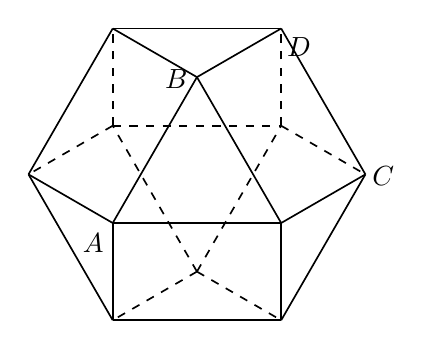
\begin{tikzpicture}[scale=0.95, semithick, every node/.style={inner sep=1.5pt}]
  % 可见棱
  \draw (-1.126,-1.950) -- (-2.252,0.000);
  \draw (-1.126,-1.950) -- (1.126,-1.950);
  \draw (-1.126,-1.950) -- (-1.126,-0.650);
  \draw (-2.252,0.000) -- (-1.126,1.950);
  \draw (-2.252,0.000) -- (-1.126,-0.650);
  \draw (1.126,-1.950) -- (2.252,0.000);
  \draw (1.126,-1.950) -- (1.126,-0.650);
  \draw (-1.126,1.950) -- (1.126,1.950);
  \draw (-1.126,1.950) -- (0.000,1.300);
  \draw (-1.126,-0.650) -- (1.126,-0.650);
  \draw (-1.126,-0.650) -- (0.000,1.300);
  \draw (2.252,0.000) -- (1.126,1.950);
  \draw (2.252,0.000) -- (1.126,-0.650);
  \draw (1.126,1.950) -- (0.000,1.300);
  \draw (1.126,-0.650) -- (0.000,1.300);
  % 被遮挡棱
  \draw[dashed] (0.000,-1.300) -- (-1.126,0.650);
  \draw[dashed] (0.000,-1.300) -- (-1.126,-1.950);
  \draw[dashed] (0.000,-1.300) -- (1.126,0.650);
  \draw[dashed] (0.000,-1.300) -- (1.126,-1.950);
  \draw[dashed] (-1.126,0.650) -- (-2.252,0.000);
  \draw[dashed] (-1.126,0.650) -- (1.126,0.650);
  \draw[dashed] (-1.126,0.650) -- (-1.126,1.950);
  \draw[dashed] (1.126,0.650) -- (2.252,0.000);
  \draw[dashed] (1.126,0.650) -- (1.126,1.950);
  % 标注：A=(0,1,1)、B=(1,1,0)、C=(1,-1,0)、D=(1,0,-1) 四个顶点
  \node[below left]  at (-1.18,-0.72) {$A$};
  \node[left]        at (-0.06,1.28) {$B$};
  \node[right]       at (2.28,-0.02) {$C$};
  \node[below right] at (1.14,1.90) {$D$};
\end{tikzpicture}
